\chapter{Beyond the Standard Model}
\label{chap:BSM}

Although the \ac{SM} represents our best understanding of the elementary particles and their interactions, it does contain some deficiencies. On the one hand, it remains silent on some important phenomena, such as gravity, dark matter, and dark energy. On the other hand, several anomalies have emerged from recent experiments, those in the flavor sector in particular. Two of the experimental results in the flavor sector that work against the \ac{SM} and their phenomenological implications are discussed in \autoref{sec:BSM}. \autoref{sec:Leptoquark} introduces the leptoquark model that can be used to explain the unexpected results that occurred in the flavor sector.

\section{BSM Phenomenology}
\label{sec:BSM}

As discussed in \autoref{sec:Flavor}, the renormalizable \ac{SM} Lagrangian exhibits a few continuous global symmetries, namely the $U(1)_{e}\bigotimes U(1)_{\mu}\bigotimes U(1)_{\tau}$ that gives rise to the conservation of lepton family numbers. Unlike gauge symmetries of the \ac{SM}, which arise at the outset of the construction, these global $U(1)$ symmetries emerge accidentally due to the assumption (massless neutrino) that is solely driven by phenomenology. Despite the accidental nature of these symmetries, they have stood up to the tests of almost all particle physics experiments to date.  

In fact, the first and so far the only hint of the broken global symmetries didn't appear until the turn of the century through the oscillation of atmospheric neutrinos \cite{Super-Kamiokande:1998kpq,SNO:2002tuh}. This remarkable observation directed significant interest from both theorists and experimentalists to the flavor sector of the \ac{SM}. On the one hand, it cements the calls for extensions of the \ac{SM} by demonstrating the mixing of neutrino flavors. On the other hand, it also suggests that the $U(1)$ symmetries are indeed broken, and the \ac{CLFV} should also occur. 

\begin{figure}[tbh!]
 \begin{center}
 \begin{tabular}{c}
 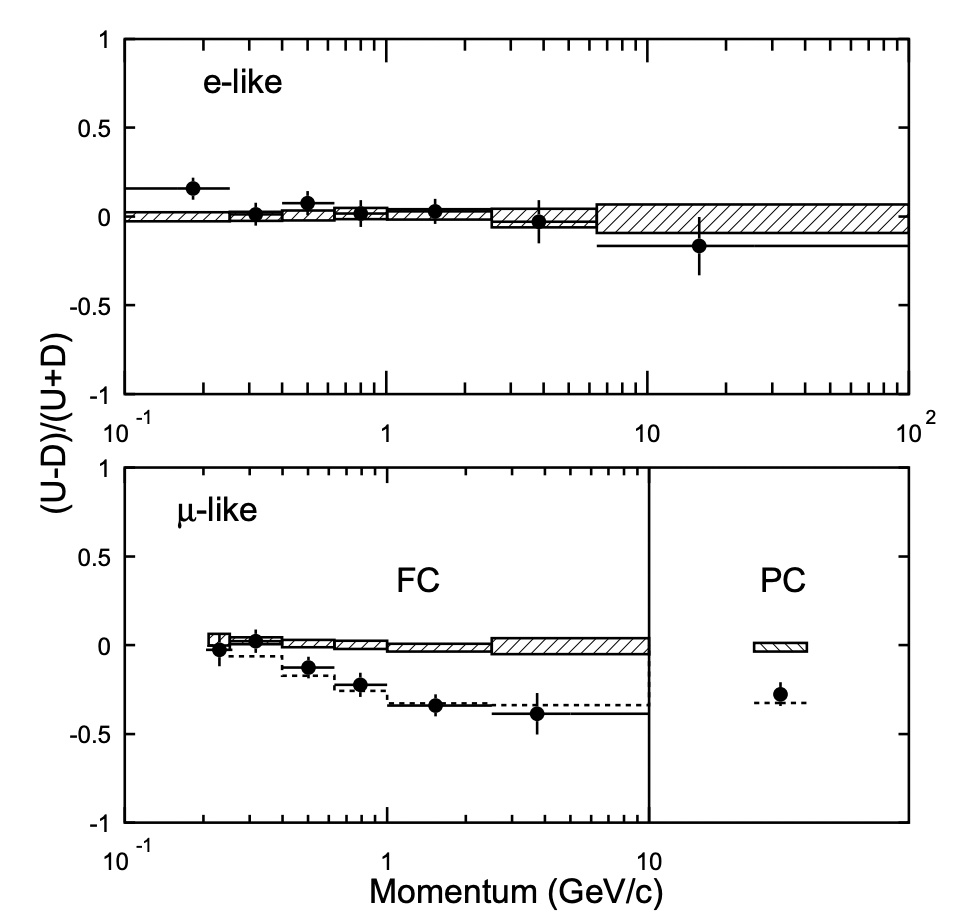
\includegraphics[width=0.6\textwidth]{figures/Part1/BSM/SuperK}
 \end{tabular}
 \caption{Evidence of neutrino oscillation presented by the Super-Kamiokande Collaboration in 1998~\cite{Super-Kamiokande:1998kpq}. The asymmetry in the zenith angle is plotted as a function of momentum for $e$-like events (upper panel) and $\mu$-like events. The data are represented with filled points. The expected distributions under the hypothesis of no neutrino oscillation are shown with filled bands while the dashed line is the expected distribution for the alternative hypothesis.}
 \label{fig:SuperK}
 \end{center}
\end{figure}

Although the exact mechanism behind neutrino mass remains unclear, it can be induced through two distinct ways that only require minimal departures from the original formulation of the \ac{SM}. By adding right-handed neutrino fields, the Yukawa coupling \cite{Weinberg:1967tq} that describes the emergence of Dirac fermion masses can be naturally extended to neutrinos. The neutrino mass can also be realized by introducing the nonrenormalizable Dimension-5 operator \cite{Weinberg:1979sa}, known as the Weinberg operator. This operator gives rise to Majorana neutrino mass terms upon spontaneous symmetry breaking. 

In either case, the masses of neutrinos are accounted for and the strength of the neutrino flavor mixing is governed by the \ac{PMNS} matrix \cite{Pontecorvo:1957cp,Maki:1962mu}, a nearly perfect analog to the \ac{CKM} matrix \cite{Cabibbo:1963yz,Kobayashi:1973fv} that describes quark mixing in the weak interaction. The same \ac{PMNS} matrix can also give rise to the \ac{CLFV} process through loop diagrams involving charged current. However, these diagrams are highly suppressed and phenomenologically negligible due to the small neutrino mass relative to the electroweak scale. Therefore, any experimental observation of \ac{CLFV} will be unambiguous evidence of new physics beyond the \ac{SM}.

Recent flavor anomalies reported by the \ac{LHCb} experiment~\cite{LHCb:2023zxo} mark the first major deviation from the SM produced by the \ac{LHC}. Not only did this result provide a direct hint towards \ac{LFUV}, it also prompted renewed experimental interest in \ac{CLFV} search since models that accommodate \ac{LFUV} generally give rise to \ac{CLFV} as well ~cite{Glashow:2014iga}. The \ac{LHC} provides the best sensitivity to \ac{CLFV} processes involving a heavy leg, such as a top quark or a Higgs boson. Moreover, some of these models~\cite{Kim:2018oih} also suggest that \ac{CLFV} involving a top quark is within the reach of the \ac{LHC} sensitivity. Therefore, a search for \ac{CLFV} in the top quark sector could shed light on these flavor anomalies and further our understanding of the broken global symmetries.

\begin{figure}[tbh!]
 \begin{center}
 \begin{tabular}{c}
 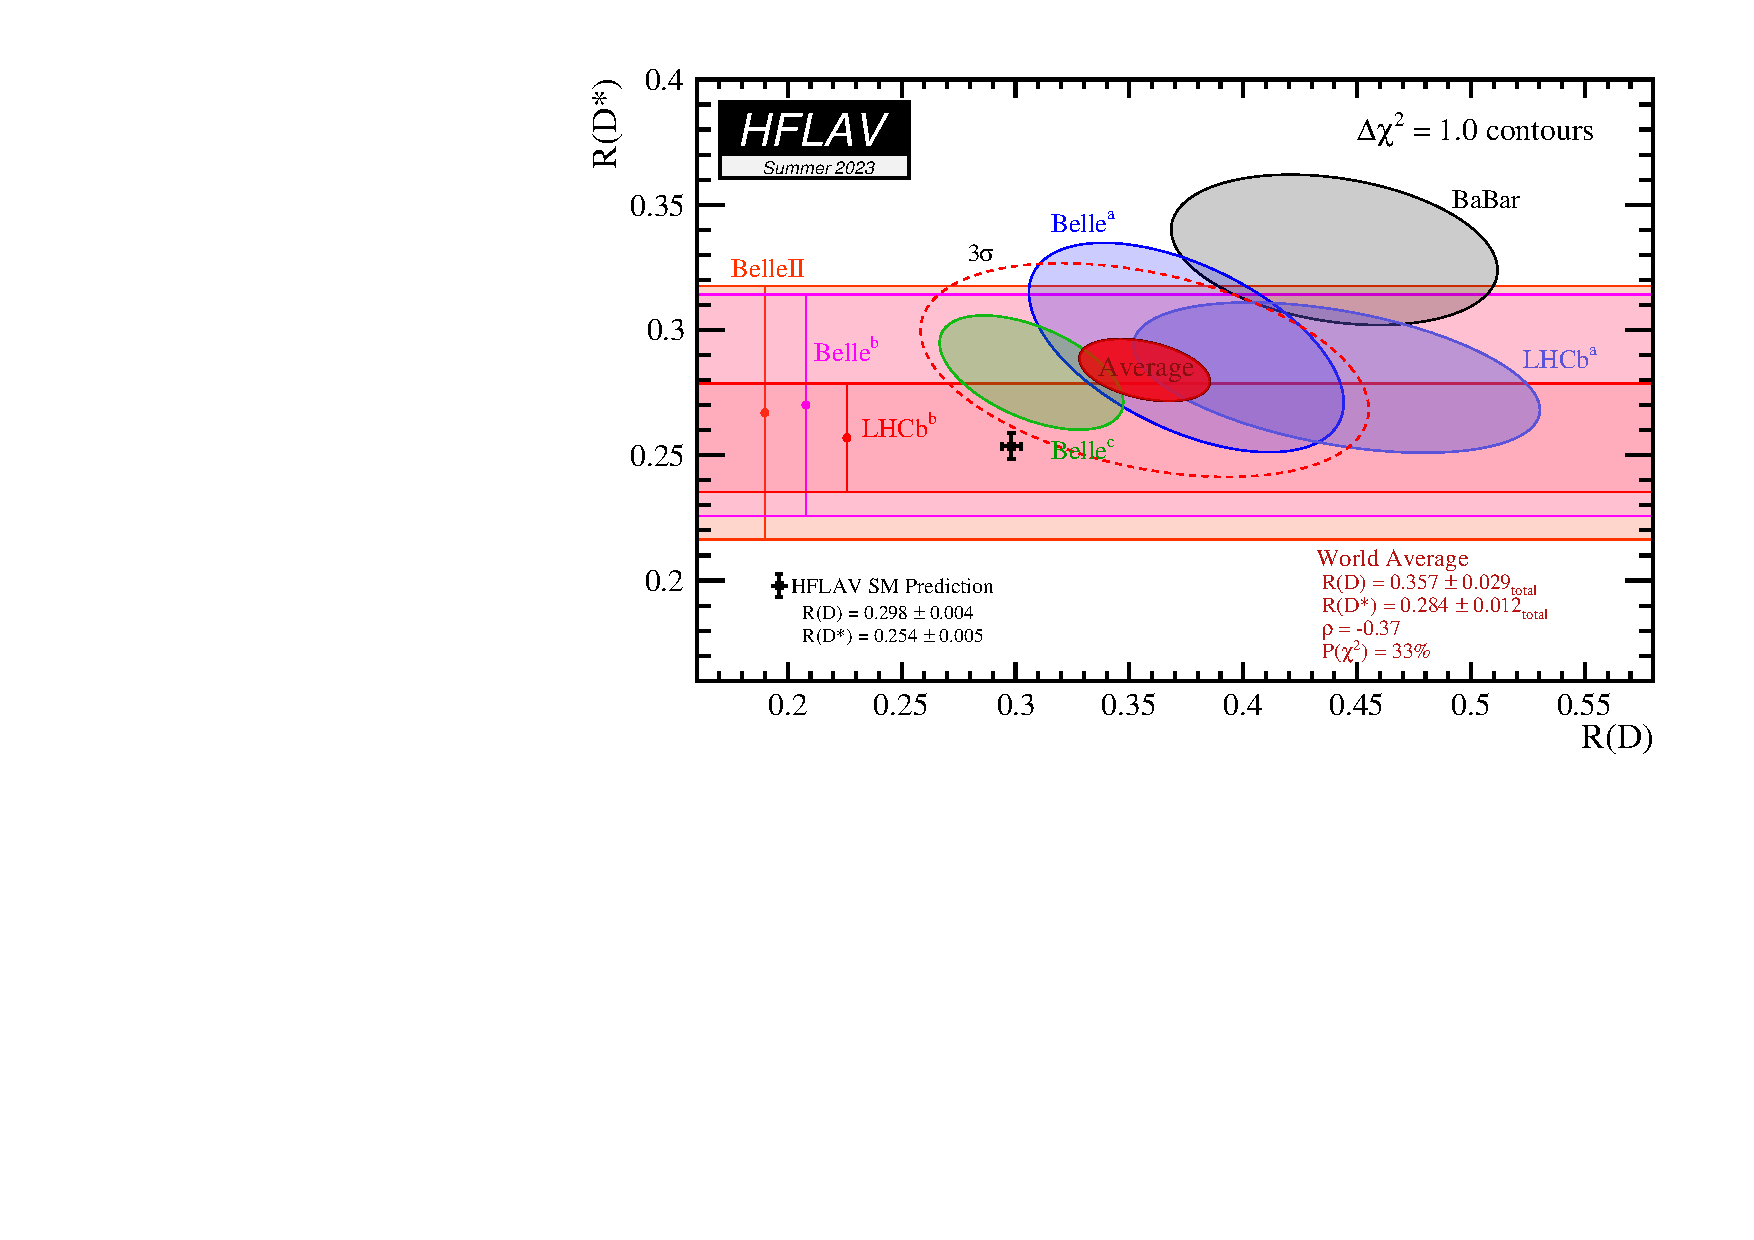
\includegraphics[width=0.7\textwidth]{figures/Part1/BSM/RD}
 \end{tabular}
 \caption{Recent results on $\mathcal{R}(D)$ and $\mathcal{R}(D^{*})$ measurements compiled by the HFLAV Group~\cite{HFLAV}. Results are shown in a two-dimensional plane with the x-axis and y-axis representing $\mathcal{R}(D)$ and $\mathcal{R}(D^{*})$, respectively. Contours with solid line boundaries represent results published by various experiments. The world average is shown in the middle. The 3$\sigma$ contour is represented with a red dashed line. The \ac{SM} prediction is represented with a data point with error bars.}
 \label{fig:RD}
 \end{center}
\end{figure}

\section{Leptoquark Model}
\label{sec:Leptoquark}

Leptoquarks are hypothetical scalar or vector bosons that were first proposed nearly half a century ago~\cite{Pati:1973uk}. They are simultaneously charged with color, isospin, and hypercharge quantum numbers, and are coupled to both leptons and quarks. When imposing the \ac{SM} \sm~gauge symmetry, a large pool of possible leptoquark candidates reduces to six scalar leptoquarks and six vector leptoquarks~\cite{Dorsner:2016wpm}, which is summarized in Table~\ref{tab:Leptoquark}. The scalar leptoquarks are: $\bar{S}_{1}$, $S_{1}$, $\tilde{S}_{1}$, $\tilde{R}_{2}$, $R_{2}$, and $S_{3}$. The vector leptoquarks are: $\bar{U}_{1}$, $U_{1}$, $\tilde{U}_{1}$, $\tilde{V}_{2}$, $V_{2}$, and $U_{3}$. 

\begin{table}[th]
\sffamily
\centering
\caption{Possible leptoquark candidates that respect \sm~gauge symmetry, summarized in Reference~\cite{Dorsner:2016wpm}.}
\begin{tabular}{cccc}
\toprule 
$(SU(3), SU(2), U(1))$ & Spin   & Symbol & Type \\ \midrule
($\bar{\bm{3}}$, $\bm{1}$, -2/3) & 0 & $\bar{S}_{1}$ & $\overline{RR}(\bar{S}_{0}^{\bar{R}})$ \\
($\bar{\bm{3}}$, $\bm{1}$, 1/3) & 0 & $S_{1}$ & $LL(S_{0}^{L})$, $RR(S_{0}^{R})$, $\overline{RR}(S_{0}^{\bar{R}})$ \\
($\bar{\bm{3}}$, $\bm{1}$, 4/3) & 0 & $\tilde{S}_{1}$ & $RR(\tilde{S}_{0}^{R})$ \\
($\bm{3}$, $\bm{2}$, 1/6) & 0 & $\tilde{R}_{2}$ & $RL(\tilde{S}_{1/2}^{L})$, $\overline{LR}(\tilde{S}_{1/2}^{\bar{R}})$ \\
($\bar{3}$, $\bm{2}$, 7/6) & 0 & $R_{2}$ & $RL(S_{1/2}^{L})$, $LR(S_{1/2}^{R})$ \\
($\bar{\bm{3}}$, $\bm{1}$, -2/3) & 0 & $S_{3}$ & $LL(S_{1}^{L})$\\
\midrule
($\bm{3}$, $\bm{1}$, -1/3) & 1 & $\bar{U}_{1}$ & $\overline{RR}(\bar{V}_{0}^{\bar{R}})$ \\
($\bm{3}$, $\bm{1}$, 2/3) & 1 & $U_{1}$ & $LL(V_{0}^{L})$, $RR(V_{0}^{R})$, $\overline{RR}(V_{0}^{\bar{R}})$ \\
($\bm{3}$, $\bm{1}$, 5/3) & 1 & $\tilde{V}_{1}$ & $RR(\tilde{V}_{0}^{R})$ \\
($\bar{\bm{3}}$, $\bm{2}$, -1/6) & 1 & $\tilde{V}_{2}$ & $RL(\tilde{V}_{1/2}^{L})$, $\overline{LR}(\tilde{V}_{1/2}^{\bar{R}})$ \\
($\bar{\bm{3}}$, $\bm{2}$, 5/6) & 1 & $V_{2}$ & $RL(V_{1/2}^{L})$, $LR(V_{1/2}^{R})$ \\
($\bm{3}$, $\bm{3}$, 1/3) & 1 & $U_{3}$ & $LL(V_{1}^{L})$\\
\bottomrule
\end{tabular}
\vspace{-0.5em}
\label{tab:Leptoquark}
\end{table}

Leptoquarks are hypothetical scalar or vector bosons that were first proposed nearly half a century ago~\cite{Pati:1973uk}. They are simultaneously charged with color, isospin, and hypercharge quantum numbers, and are coupled to both leptons and quarks. When imposing the \ac{SM} \sm~gauge symmetry, a large pool of possible leptoquark candidates reduces to six scalar leptoquarks and six vector leptoquarks~\cite{Dorsner:2016wpm}, which is summarized in Table~\ref{tab:Leptoquark}. The scalar leptoquarks are: $\bar{S}_{1}$, $S_{1}$, $\tilde{S}_{1}$, $\tilde{R}_{2}$, $R_{2}$, and $S_{3}$. The vector leptoquarks are: $\bar{U}_{1}$, $U_{1}$, $\tilde{U}_{1}$, $\tilde{V}_{2}$, $V_{2}$, and $U_{3}$. 

Leptoquarks are hypothetical scalar or vector bosons that were first proposed nearly half a century ago~\cite{Pati:1973uk}. They are simultaneously charged with color, isospin, and hypercharge quantum numbers, and are coupled to both leptons and quarks. When imposing the \ac{SM} \sm~gauge symmetry, a large pool of possible leptoquark candidates reduces to six scalar leptoquarks and six vector leptoquarks~\cite{Dorsner:2016wpm}, which is summarized in Table~\ref{tab:Leptoquark}. The scalar leptoquarks are: $\bar{S}_{1}$, $S_{1}$, $\tilde{S}_{1}$, $\tilde{R}_{2}$, $R_{2}$, and $S_{3}$. The vector leptoquarks are: $\bar{U}_{1}$, $U_{1}$, $\tilde{U}_{1}$, $\tilde{V}_{2}$, $V_{2}$, and $U_{3}$. 

\begin{figure}[tbh!]
 \begin{center}
 \begin{tabular}{cc}
 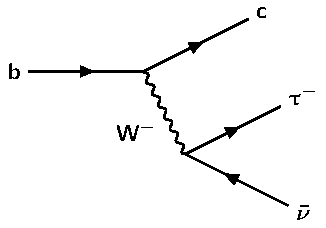
\includegraphics[width=0.45\textwidth]{figures/Part1/BSM/SMbtoc}&
 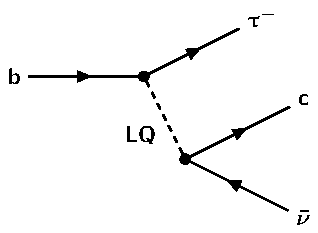
\includegraphics[width=0.45\textwidth]{figures/Part1/BSM/Leptoquark}\\
 \end{tabular}
 \caption{Representative Feynman diagram for tree-level $\textsf{b}\rightarrow\textsf{c}\uptau\nu$ transition. The \ac{SM} contribution is shown on the left. Possible contributions from leptoquarks, denoted by LQ in the diagram, are shown on the right.}
 \label{fig:Leptoquark}
 \end{center}
\end{figure}

Leptoquarks are hypothetical scalar or vector bosons that were first proposed nearly half a century ago~\cite{Pati:1973uk}. They are simultaneously charged with color, isospin, and hypercharge quantum numbers, and are coupled to both leptons and quarks. When imposing the \ac{SM} \sm~gauge symmetry, a large pool of possible leptoquark candidates reduces to six scalar leptoquarks and six vector leptoquarks~\cite{Dorsner:2016wpm}, which is summarized in Table~\ref{tab:Leptoquark}. The scalar leptoquarks are: $\bar{S}_{1}$, $S_{1}$, $\tilde{S}_{1}$, $\tilde{R}_{2}$, $R_{2}$, and $S_{3}$. The vector leptoquarks are: $\bar{U}_{1}$, $U_{1}$, $\tilde{U}_{1}$, $\tilde{V}_{2}$, $V_{2}$, and $U_{3}$. 